\documentclass{article}
\usepackage{amsmath}
\usepackage{amsthm}
\usepackage{amsfonts}
\usepackage{amssymb}
\usepackage{color}
\usepackage{latexsym}
\usepackage{listings}
\usepackage{epsfig}
\usepackage{graphicx}
\usepackage{cite}
\usepackage[all]{xy}
\usepackage{fullpage}
\usepackage[left=1in,top=1in,right=1in,bottom=1in]{geometry}

\theoremstyle{definition}
\newtheorem{definition}{Definition}
% spellcheck using ``aspell -c filename'' in Unix
\title{The Parallax Programming Model and Language}
\author{Michael Bauer, Sean Treichler, Alex Aiken}

%%%%%%%%%%%%%%%%%%%%%%%%%%%%%%%%%%%%%%%%%%%%%%%%%%%%%%%%%%%%%%%%%%%%%%%%%%%%%%%%

\lstset{ %
	language=C++,                % choose the language of the code
	basicstyle=\footnotesize,       % the size of the fonts that are used for the code
	numbers=left,                   % where to put the line-numbers
	numberstyle=\footnotesize,      % the size of the fonts that are used for the line-numbers
	stepnumber=1,                   % the step between two line-numbers. If it's 1 each line will be numbered
	numbersep=5pt,                  % how far the line-numbers are from the code
	backgroundcolor=\color{white},  % choose the background color. You must add \usepackage{color}
	showspaces=false,               % show spaces adding particular underscores
	showstringspaces=false,         % underline spaces within strings
	showtabs=false,                 % show tabs within strings adding particular underscores
	frame=single,	                % adds a frame around the code
	tabsize=2,	                % sets default tabsize to 2 spaces
	captionpos=b,                   % sets the caption-position to bottom
	breaklines=true,                % sets automatic line breaking
	breakatwhitespace=false,        % sets if automatic breaks should only happen at whitespace
	title=\lstname,                 % show the filename of files included with \lstinputlisting; also try caption instead of title
	escapeinside={\%*}{*)},          % if you want to add a comment within your code
	morekeywords={tunable, }            % if you want to add more keywords to the set
}

%%%%%%%%%%%%%%%%%%%%%%%%%%%%%%%%%%%%%%%%%%%%%%%%%%%%%%%%%%%%%%%%%%%%%%%%%%%%%%%%

\begin{document}

\maketitle
\pagebreak

\tableofcontents
\pagebreak

%%%%%%%%%%%%%%%%%%%%%%%%%%%%%%%%%%%%%%%%%%%%%%%%%%%%%%%%%%%%%%%%%%%%%%%%%%%%%%%%
% Introduction 

\section{Introduction \label{Intro}}
% Multicore revolution
% Memory-compute mismatch
% Hieararchical memory
% Locality-aware programming systems
% Regions for locality and independence

\subsection{Related Work \label{Related}}

\subsubsection{Locality-Aware Programming Models \label{LocalityAware}}
% Chapel
% X10/Hiearchical Place Trees
% Sequoia

\subsubsection{Region Languages \label{RegionLangs}}
% Re-heaps
% RC
% Cyclone

\subsection{Outline \label{Outline}}

\subsection{Document Scope and Completeness \label{Scope} }
The scope of this document is the design of the Parallax programming model
as well as some of the syntax of the Parallax language.  We describe in a 
separate document the implementation of a Parallax compiler and runtime system
capable of supporting the Parallax language.  Not all features and interactions
for the language have been fully specified.  Some outstanding issues are listed
in Section \ref{OutstandingQs}.

\pagebreak

%%%%%%%%%%%%%%%%%%%%%%%%%%%%%%%%%%%%%%%%%%%%%%%%%%%%%%%%%%%%%%%%%%%%%%%%%%%%%%%%
% Motivation

\section{Motivating Applications \label{Applications}}
% The need for applications to drive research
% Applications other than arrays
% Ghost cells
% Recursive decomposition for hierarchical memory

% Mesh based applications
% Graph algorithms
% Tree data structures
\noindent
The motivation for creating the Parallax programming model and language came
directly from a class of applications that we found difficult to describe
using other parallel languages.  The characteristics of these applications were that
they all required distributed pointer data structures.  Furthermore these pointer data
structures could not easily be represented by arrays due to either irregularity
in the data structure or complex sharing patterns.  These characteristics
prevent us from using array-centric languages like Sequoia \cite{Fatahalian06} 
or Chapel \cite{Chamberlain07} to implement these applications and still
achieve high performance. \\

\noindent
To better understand this set of applications we have constructed a
classification of the various applications that we've encountered.  The
classification is determined primarily based on the data structures used in
the applications as opposed to the kind of parallelism that exists.  This
is a direct consequence of our goal to build locality-aware languages instead
of simply parallel languages.  To reason about the locality present in
application we must consider the data structures required for an application.\\

\noindent
In this section we will first describe the set of data structure classes
that we are interested in supporting in Parallax.  We then present two example
applications that will be used as running examples throughout this document
to illustrate important Parallax concepts.

\subsection{Data Structure Classification \label{DataStructures}}
\noindent
There are three primary classes of data structures that we are interested
in investigating in Parallax: meshes, graphs and trees.  These classes of data 
structures are not intended to be representative of all applications for
our targets machines.  However, we believe that they capture a 
much larger set of applications than could have been described in previous
languages.  We now define each of these data structure classes and provide
instances of applications that use these data structures.

\subsubsection{Meshes \label{Mesh}}
\noindent
The first set of applications that motivated our design of Parallax was 
applications which made use of mesh based data structures.  We define a mesh
to be any data structure which consists of a polygonal structures which we
call {\tt cells}.  These polygonal structures can exist in any number of dimensions.
The only requirement of cells is that they have a neighbor relationship which
operates as a manifold in the formal mathematical sense.  This allows us
to differentiate meshes from graphs described in Section \ref{Graphs} and indeed
the locality properties of these two classes of data structure are very 
different.  Meshes may also have shared sub-structures (i.e. two cells sharing
a face or an edge), but this isn't a necessary condition for a mesh. \\

\noindent
Given this description of a mesh, we believe that there are several different
sub-classes of applications that use mesh based data structures.  We break
these sub-classes down across two different dimensions:

\begin{enumerate}
\item Regular/Irregular - Formally we'll classify a mesh as regular if the basis
of the vector space corresponding to the neighbor relationship manifold is the same
for all cells in the mesh and irregular otherwise.  Intuitively, if there is 
a $O(1)$ function in time and space for computing the neighbor relationship for 
all cells in the mesh we'll classify the mesh as regular.
\item Gather/Scatter - This is a property of the computation being performed on
the mesh and determines whether or not the operation on a single cell requires
only reading neighbor cells (gather) or reading and writing neighbor cells (scatter).
\end{enumerate}

\noindent
Given these different dimensions for classifying mesh data structures and mesh
computations we can now give examples of computations that fit in each category.

\begin{center}
\begin{tabular}{|c||c|c|}
\hline
 & Regular & Irregular \\ \hline \hline
Gather & Reverse-Time Migration \cite{Micikevicius09} & Lattice-Boltzmann \cite{Heuveline07} \\ \hline
Scatter & Fluidanimate \cite{Bienia08} & Liszt DSL\cite{DeVito10} \\ \hline
\end{tabular}
\end{center}

\begin{itemize}
\item Reverse-Time Migration - This application relies on a mesh that consists of
a three dimensional array.  For each time step only reads of neighboring cells are
required to perform a computation.
\item Lattice-Boltzmann - Lattice-Boltzmann computations can involve either
regular or irregular meshes, but computations to update a cell for a given time
step involve gathering (reading) information from neighboring cells.
\item Fluidanimate - An application from the Parsec Benchmark Suite \cite{Bienia08}
that relies on a three dimensional array of cells, but scatters updates to
neighboring cells rather than reading from neighboring cells.
\item Liszt DSL - A domain specific language for mesh-based partial differential
equations.  Meshes can be either regular or irregular, but updates are scattered
to neighboring cells often with specific reduction phases.
\end{itemize}

\noindent
These applications are just a sampling of the many codes that could be 
classified under these sets of mesh computations.  Our goal in designing
Parallax is to be able to handle applications that fit under all four of
these classes of mesh based computations.

\subsubsection{Graphs \label{Graphs}}
\noindent
Another class of data structures that we want to be able to handle in Parallax
are graph data structures.  Graphs differ from meshes as the
notion of a neighbor relationship in graphs do not have to obey any nice 
mathematical requirements.  Instead nodes in a graph are neighbors
if they simply share an edge which makes it much more difficult to identify
locality in graph data structures.  Due to this property we have chosen
to separate applications which use graph data structures into a
separate class of applications. \\

\noindent
One current thinking on graph applications is that there are two classes of
graph applications \cite{Bader11}:

\begin{itemize}
\item Static Graph Algorithms - operate on graphs which once
loaded into an application do not change for the duration of the program.
\item Dynamic Graph Algorithms - operate on graphs which can change 
throughout the duration of a computation with new inputs, or modifications
to the graph by the algorithm itself.
\end{itemize} 

\noindent
These two classes of graph algorithms will require different graph 
representations.  In the case of static graph algorithms, the graph
can be partitioned at load-time, while for dynamic graphs there may need
to be load balancing steps to move parts of the graph data structure
around at runtime.  Another goal of Parallax is to be capable of handling
both classes of graph algorithms and data structures.

\subsubsection{Trees \label{Trees}}
\noindent
The last class of data structures that we want to be able to support
with Parallax are tree data structures.  Trees are a special type of
graph data structure in which the locality is very clear.  Tree data
structures tend to be highly scalable in parallel environments due to 
their obvious division of work between independent sub-trees.  Tree
data structures also mirror the underlying memory hierarchy of parallel
machines which is often structured as a tree.\\

\noindent
While there are not many scientific applications which rely on tree
data structures, there are interesting parallel applications which use
tree data structures.  Other members of our research group are interested
in performing static analysis over large abstract syntax trees, often
describing multi-million line programs like the Linux kernel \cite{Dillig10}.
Many of these static analyses can be performed in parallel, but require
significant amounts of memory and benefit from being run over large machines
which can handle their working sets.  Handling tree data structures
for applications such as these is another Parallax goal.

\subsection{Simple Example Application: Linked List Fold \label{LinkedList}}
\noindent
In this section and the next we introduce two applications that will serve to
be running examples throughout the remainder of the document.  This first
example application is trivial and will only be used to illustrate basic
concepts.  The example in section \ref{GraphSim} will be used to demonstrate
the need for more advanced concepts and how the language actually works.\\

\noindent
Our simple example application has a single data structure consisting of a
linked list of integers.  Each node in the linked list contains a single integer
and a pointer to the next element in the linked list.  The computation that
we wish to perform over the linked list is a fold reduction to compute the 
sum of the linked list. \\

\noindent
Our goal is to be able to parallelize this computation for an arbitrarily
deep hierarchical memory machine.  To do so we want to be able to 
partition the linked list into independent sub-lists and then potentially
continue partitioning sub-lists for as many levels of the memory hierarchy
as necessary.  Ultimately a sequential summation will be performed on
each sub-list and results reduced by the tree of parent computations.

\subsection{Advanced Example Application: Graph Based Simulation \label{GraphSim}}
\noindent
As an example of a more advanced application inline with the different sets
of applications that we introduced in section \ref{DataStructures} we now
describe a graph based simulation.  This particular application is an instance
of a static graph application described in section \ref{Graphs}. \\

\noindent
Our application takes as input a large graph representing an electrical
circuit\footnote{This is what happens when two electrical engineers
design a programming model.}.  The nodes in the graph represent points of
constant voltage or connections between circuit elements.  The edges of
the graph represent circuit elements including voltage sources, current
sources, resistors, capacitors, and inductors.  The application then
simulates this circuit using Kirchhoff's current and voltage laws for
a large number of time steps.\\

\noindent
To perform this computation in parallel we will have to partition this graph
into sub-graphs.  For hierarchical memory we will want to recursively partition
the graph an arbitrary number of times.  Once we have partitioned the graph at the beginning
of the computation, we can then perform the simulation in a two phase approach.
In the first phase, each partition gets the most up to date information from
adjacent nodes that are not in the partition.  The second phase then uses
this information to simulate the local partition.  This can be done at every
level of partitioning.  Each phase is performed for every time step
of the simulation.

\pagebreak

%%%%%%%%%%%%%%%%%%%%%%%%%%%%%%%%%%%%%%%%%%%%%%%%%%%%%%%%%%%%%%%%%%%%%%%%%%%%%%%%
% Regions

\section{A Region Programming Model \label{Regions}}
% Goals of region programming model

\noindent
In this section we propose a new region-based programming model for describing
computations to be performed on hierarchical memory machines.  
While our ultimate goal is to design a parallel language, we've explicitly
decoupled the region programming model from our model of parallelism.  Our region
programming model doesn't require parallelism to describe locality.  We even believe
it could be beneficial for exploiting locality in a sequential language as described
in section \ref{Sequential}. \\

\noindent
The primary difference between previous programming models and our region programming
model is its model of memory.  Most traditional programming models use the
abstractions of a globally visible heap (shared memory) and a stack for each thread
of control.  In distributed programming models there are independent heaps for each
process of control (MPI).  Instead of relying on these abstractions that are tied
to the machine, we raise the level of abstraction in how memory is managed.\\

\noindent
In our model all memory is allocated inside of a set of regions which are explicitly
under the control of the programmer.  We feel that regions and the operations on them
that we describe in this section are sufficient to provide the following information:

\begin{enumerate}
\item Locality - regions should be capable of describing data that
should be colocated for a computation to be performed.
\item Independence - regions should enable us to reason about which computations
use disjoint data and can be run independently.
\item Pointer Fidelity - to ensure independence and enable us to move regions
throughout the memory hierarchy we need to know exactly which regions pointers target.
\end{enumerate} 

\noindent
More importantly this information can be conveyed by our region programming model in
a machine agnostic context.  This will allow the compiler, runtime system, and the
programmer to specify how to map region programs to different hierarchical memory
machines at a later period of time as described in section \ref{Mapping}. \\

\noindent
To introduce our region programming model, we first provide definitions and concepts
required for understanding our definition of regions.  We then describe the 
operations that the programmer is capable of performing on regions.  Next we
describe the need for region relationships.  Finally, we show how arrays
are just a special case of regions.

\subsection{Region Definition \label{RegionDef}}
% Basic definitions required for defining regions
\noindent
To describe our region programming model we first need to define some common terms
that will be used throughout our programming model description.  
We begin by defining an allocation and a pointer to an allocation.  
From these definitions we can then define a region.

\begin{definition}
An {\tt allocation} is a pair ($T$,$R$) where $T$ is an instance of a type $T$ from
the type system and $R$ is a region. 
\end{definition}

\begin{definition}
A {\tt pointer} of type $T$ into a region $R$ is a reference to a unique allocation
of type $T$ in region $R$.
\end{definition}

\noindent From these definitions we can now specify our definition of a region.

\begin{definition}
A {\tt region} $R$ is a potentially empty mapping of pointers to allocations of type 
$T$ in region $R$.  All allocations (and therefore all pointers) in a region must be of the
same type $T$.  This restriction is necessary for guaranteeing the type safety of 
pointers into the region\footnote{It also has an added implementation benefit described
in the technical report on the implementation the Parallax compiler and runtime system.}.
\end{definition}

\noindent
Unlike previous work on regions (see section \ref{RegionLangs}), our 
definition of a region is independent of the hardware we are targeting.  
We don't rely on the concept of memory pages anywhere in our definition of 
a region.  Our definition of a region is simply an abstract  mapping that 
enables us to use pointers to uniquely identify allocations.  We can
describe locality using regions by placing two allocations in the same region.
We can also describe data independence by performing two allocations in different
regions. \\

\noindent
From our definition of a region we can now define a sub-region relationship.

\begin{definition}
A region $R$ is said to be a {\tt sub-region} or {\tt child region} of a parent region $P$
if the mapping for $R$ is a subset of the mapping for $P$.
\end{definition}

\noindent
The sub-region relationship will be critical for providing the ability 
to recursively decompose data structures contained within a region.  Our approach
will allow us to mirror the way that the Sequoia language was able to recursively 
decompose arrays.  We describe in more detail how to create sub-regions in Section
\ref{RegOp}. \\

\subsection{Region Operations \label{RegOp}}
% Basic operations on regions
\noindent
There are three complementary pairs of region operations that are available to a
programmer.  The first two pairs of operations are basic operations on regions 
that allow the programmer to create/destroy regions and to allocate/free memory
inside of a region.  The third pair of operations partition/union allow for the recursive
decomposition of data structures into sub-regions.

\subsubsection{Creation and Destruction \label{CreateDestroy}}
\noindent
To be able to allocate memory the programmer must first have the ability to create
and destroy regions.  There are built-in calls to the language for creating a region
and destroying a region.  The call to create a region must take as a parameter the
type of region to create and then returns a unique region identifier.  The type
passed to a call to create a region can either be any type in the type system 
or a region relationship (described in more detail in section \ref{RegionRelationship}).
If the type passed is a type from the type system then the region identifier
is simply a handle, but if the type is a region relationship, then the region
identifier will have region handles for each of the regions in the region relationship. \\

\noindent
To delete a region the programmer calls a delete region function that takes
as an argument a region identifier.  Memory management of regions is explicit and
it is therefore possible to have memory leaks if a program does not delete
regions before their handles go out of scope.\\

\noindent
Regions are not first class objects and therefore region identifiers have a special
type that is not permitted to be written into memory or read out of memory.  This
restriction is enforced by the type system.  We may consider in the future making
regions first class objects, but to simplify our region analysis we currently
don't permit this.

\subsubsection{Allocation and Deletion \label{AllocDelete}}
\noindent
The only way to allocate memory in our programming model is to allocate it inside
of a region.  Calls to malloc and free in our language take a region in which to
perform an allocation.  Since the region is already typed with the type of element
that it contains, then a call to malloc on a given region will return a pointer to
an allocation of the given region's type.  The type of the returned pointer is
also qualified to point into region in which the allocation was performed. \\

\noindent
Allocation also has an interesting interaction with sub-region relationships.  If
an allocation is performed in a region that is a sub-region of a parent region
then the allocation is also added as a valid allocation of the parent region.  This
follows directly from our definition of sub-region given in section \ref{RegionDef}:
the mapping from pointers to allocations for a sub-region must be a subset of the
mapping of its parent.  This allocation operation is transitive which implies that
an allocation in any sub-region will automatically be valid in any of the ancestor
regions of the region in which the allocation was performed. \\

\noindent
Unlike allocation, deleting an element from a region does not have the same effect
as allocation of applying to any ancestor region.  Instead deletion operates on
all sub-regions of the region in which the deallocation is performed.  To understand
the reasoning behind this consider the following scenario: an allocation is performed in a
parent region and is added to two different sub-regions of the parent region (we
describe how this occurs in section \ref{Partition}).  If we delete the allocation
from one of the sub-regions, we cannot safely delete the allocation from the parent region
because the allocation is still valid in the other sub-region.  However, if we delete
the allocation from the parent region, then we must delete the allocation from all of
the child regions to maintain the definition of a sub-region relationship.

\subsubsection{Partition \label{Partition}}
\noindent
To this point we have only provided basic operations on regions that are a part of
any region language.  This section introduces the first of two operations that give us the
machinery necessary for describing how to recursively decompose data structures in
regions.  The first operation, partition, will take a region and break
it apart into a set of sub-regions.  Conversely the second operation, union, will
take two sub-regions with a common ancestor and allow us to combine them into a
new region and is described in section \ref{Union}. 

\noindent
To describe how partitioning of a region is performed we first introduce the
concept of a coloring and several properties of a coloring.

\begin{definition}
A {\tt coloring} is a mapping from a (sub)set of pointers valid in a region
to $\mathbb{N}$.  The subset of $\mathbb{N}$ in the image of the mapping
is called the set of {\tt colors} used in the coloring.
\end{definition}

\begin{definition}
A coloring is said to be {\tt disjoint} if the color mapping is injective, otherwise
the coloring is said to be {\tt aliased}.
\end{definition}

\begin{definition}
A coloring is said to be {\tt total} if the color mapping is surjective, otherwise
the coloring is said to be {\tt subtotal}.
\end{definition}

\noindent
The process of creating a partition is a two step process.  In the first
step the programmer is responsible for creating the coloring.  In the second step
the programmer then invokes a built-in partition functioning that takes as
arguments the original region, the coloring, and the set of colors used to
create the coloring.  The built-in partitioning function then returns a
special data structure called a collection of regions.

\begin{definition}
A {\tt region collection} is a special data structure that holds the set
of sub-regions returned by a partitioning operation and can be indexed by
the set of colors used in the partitioning.  The type of a region collection
is also qualified by the properties of coloring that created it such
as disjoint/aliased and total/subtotal. 
\end{definition}

\noindent
It is legal for there to be more than one partition made of a region.  This allows
the programmer to use different partitions of a data structure during different
phases of a computation when different locality properties of the data structure
might be exploited.  The ability to have multiple views into a data structure by
creating separate partitions creates a parallax on the data structure.\footnote{This 
is the naming origin of our language.}\\

\noindent
To make the concept of a partitioning concrete we now describe how partitioning
works for both of the example programs introduced in section \ref{Applications}.
For the case of the linked list we create a coloring that maps allocations in
contiguous ranges of the linked list to different sub-regions as can be
seen in figure \ref{fig:LinkedListColor}.  We can then pass
this coloring to the partition function that will return a region collection consisting
of the green, blue, and red sub-regions of the initial region. \\

\begin{figure}[t]
\centering
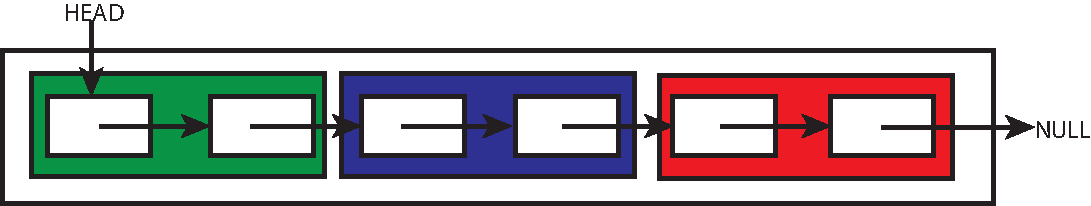
\includegraphics[width=4in]{figs/LinkedListPartition.pdf}
%\vspace{-5mm}
\caption{Coloring for partitioning a linked list. \label{fig:LinkedListColor}}
\end{figure}

\noindent
To describe the sharing scheme for the circuit simulation we will need
multiple partitions.  Recall from section \ref{GraphSim} that we want to
partition up the graph in such a way that we can keep track of which nodes
have to be shared with other subsets of the graph so we can exchange information
as dictated by the first phase of the graph algorithm.  To do this we first want
to partition the graph into the nodes that are private to computations
and those that are shared between computations.\\  

\noindent
Figure \ref{fig:GraphPartition}
shows the view of a set of nodes in the graph from the perspective of a
computation.  In this figure all the nodes inside the black circle
are nodes that the computation owns, while all the nodes outside the orange circle
are nodes that are shared between different computations.  This creates three
different sets of nodes that must be created from the set of all nodes: private
to a computation, owned by a computation but shared, and then read by a computation
but owned by a different computation. \\

\begin{figure}[t]
\centering
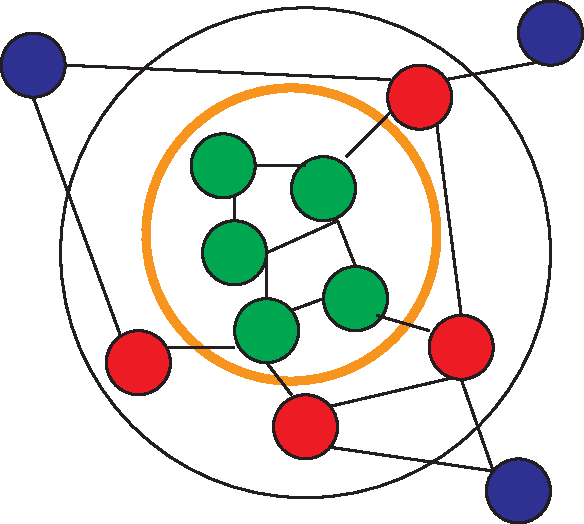
\includegraphics[width=4in]{figs/GraphPartition.pdf}
\caption{A subset of the circuit simulation graph from the perspective of
a computation.  Nodes inside of the black circle are owned
by the computation.  Nodes outside of the orange circle are shared between
computations.  There are then three different sets of nodes that must be
described: private to a computation (green), owned and shared (red), and
not owned but read (blue). \label{fig:GraphPartition}}
\end{figure}

\noindent
To create the sets described in figure \ref{fig:GraphPartition} we will
need several partitions of the set of nodes.  To show the different partitions
visually we have created a symbol to represent the partition operator which
can be seen in figure \ref{fig:PartitionOperator}.  The partition operator
indicates that a region should be partitioned into a set of sub-regions.  The
$N$ in figure \ref{fig:PartitionOperator} indicates the number of sub-regions
which will be created.  The partition operator can also specify whether the
partition is disjoint/aliased and total/subtotal.\\

\begin{figure}[t]
\centering
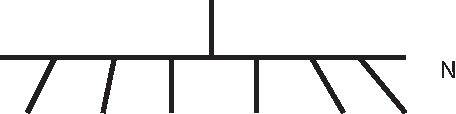
\includegraphics[width=3in]{figs/PartitionSymbol.pdf}
\caption{Symbol for a partition of a region into sub-regions.  The $N$
indicates the number of sub-regions to be created. \label{fig:PartitionOperator}}
\end{figure}

\noindent
The different partitions that are required to break up the set of all nodes
in the graph can now be seen in figure \ref{fig:GraphPartitionGraph}.  We
first partition the nodes into two sub-regions: those nodes which are private
to computations and those which are shared between computations.  This
corresponds to the orange circle in figure \ref{fig:GraphPartition} and
the orange partition in figure \ref{fig:GraphPartitionGraph}.  For the 
private sub-region we can again partition this region into the sets of private
nodes for each computation corresponding to the green nodes in figure 
\ref{fig:GraphPartition} and the green partition in figure
\ref{fig:GraphPartitionGraph}.\\

\begin{figure}[t]
\centering
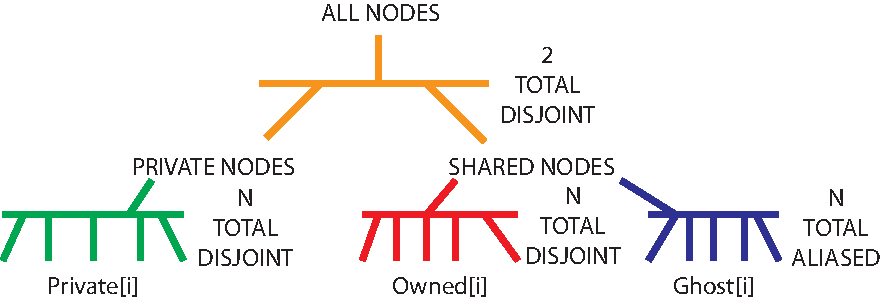
\includegraphics[width=4in]{figs/GraphPartitionGraph.pdf}
\caption{Illustration of the different partitions required for
breaking up the set of nodes in the circuit application.
\label{fig:GraphPartitionGraph}}
\end{figure}

\noindent
For the shared sub-region, we now want to partition this group of nodes two
different ways, one to capture the set of a nodes that are shared by computations
but still owned, and one to capture the set of nodes that are not owned but
required for a computation.  We create a separate partition of all the shared
nodes to describe each of these sets.  The first partition to describe the owned
nodes is over all $N$ computations and is therefore total and disjoint because each shared
cell can only belong to one computation.  This partition corresponds to the
red nodes in figure \ref{fig:GraphPartition} and the red partition in figure
\ref{fig:GraphPartitionGraph}.  The second partition to describe the set of nodes
that have to be read but are not owned (ghost nodes), is over all $N$ computations
and corresponds to the blue nodes in figure \ref{fig:GraphPartition} and the blue 
partition operator in figure \ref{fig:GraphPartitionGraph}.  This partition is
total but aliased because all the shared nodes are ghost nodes for at least one
other computation, but can also be ghost nodes for multiple other computations.\\

\noindent
This example has demonstrate the power of the partitioning operation as it's shown
that we can capture complicated sharing patterns using multiple partitions.  The
ability partition regions isn't enough however if we want to be able to recursively
decompose data structures.  To achieve our goal of an arbitrary level of 
decomposition we need an additional operation as shown in the next section.

\subsubsection{Union \label{Union}}
\noindent
In this section we introduce the union operation as a complementary operation
to the partition operation.  To understand the need for a union operation consider
the graph-based circuit simulation from section \ref{GraphSim}.  In section \ref{Partition}
we described how to partition the graph of nodes ONE time, but our goal is to
be able to partition it as many times as necessary for hierarchical memory.  To
achieve this goal we need to be able to maintain a recursive invariant.\\

\noindent
Our initial computation wanted to partition a single set of nodes but after
the partitioning from section \ref{Partition} each computation now has three
sets of nodes: private, owned, and ghost.  Each of these computations may want
to again partition the set of nodes for which it is responsible.  In the
case of the circuit simulation this is the set of private nodes unioned with
the set of owned nodes.  To achieve this we provide a union operation to create
a new region which is the result of a union between two regions.  For the circuit
simulation we can then pass the result of this union operation to function
which performs the partitioning and recursively decompose our graph as many times
as necessary.  This recursive invariant can be seen in figure \ref{fig:UnionPartition}
where we apply a union for each pair of shared and private nodes to get a new
subset of the graph.  Note that because we maintained disjoint/aliased and
total/subtotal information about each partition we can infer that the region
collection resultant from unioning together {\tt Private[i]} and {\tt Owned[i]}
is both disjoint and total. \\

\begin{figure}[t]
\centering
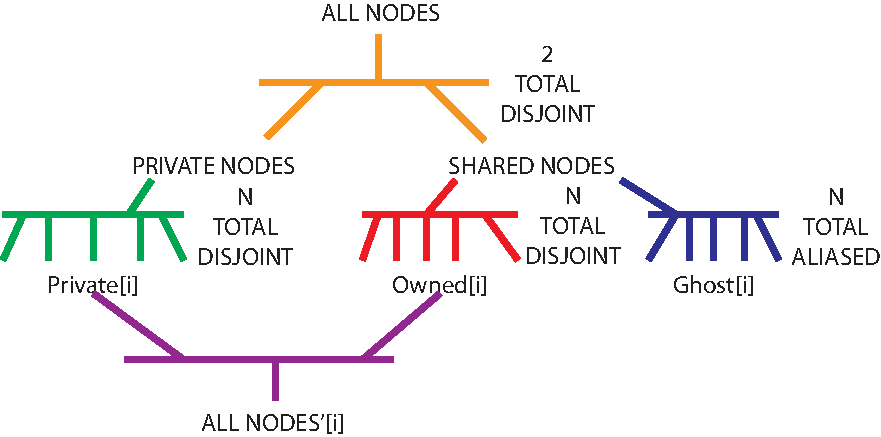
\includegraphics[width=4in]{figs/UnionPartitionGraph.pdf}
\caption{Illustration of the union operator on regions to restore the recursive
invariant of a single set of nodes in the circuit graph simulation. \label{fig:UnionPartition}}
\end{figure}

\noindent
The only rule for region union is that the two regions being unioned must share
a common ancestor.  This is important for maintaining the invariants specified
by the sub-region relationship.  The created region is a parent region to
each of the unioned child regions and a child region of the least common ancestor
of the set of regions which were unioned together.  By adding the ability to perform region
unions we can no longer describe the set of all region relationships using a tree
like all previous region languages, but instead require a directed acyclic graph
to describe all the regions.  Note that this still maintains the sub-region
relationship we defined in section \ref {RegionDef}.

\subsection{Region Relationships \label{RegionRelationship}}
% Mutually recusive region relationships
\noindent
As stated at the beginning of this section one of the goals of our programming model
is to accurately model the set of regions a pointer can target.  To do this we
qualify every pointer type with a set of regions into which it can point.  By also
restricting regions to only contain allocations of a single type, we can parametrize
the type of the allocation on the region on which it is contained.  This can give us
very strong guarantees about where pointers within a region can point.\\

\noindent 
Consider the linked list example from section \ref{LinkedList}.  In this case we create
a region which will contain allocations of linked list nodes.  Our system however allows
us to guarantee that the pointers to the next element in every linked list
node also point into the same region in which the allocation occurs because we can
parameterize the type of allocations in the region on the region itself.  This allows
the compiler to reason about locality in this data structure by specifying that all
the nodes in the linked list are in a single region.\\

\noindent
The approach illustrated above works well when an entire data structure can be
represented by a single type in a single region.  However, many data structures require
multiple types to represent and often these types are self referential.  Consider
the case of the graph example from section \ref{GraphSim}.  In this example there
are two types to this data structure: nodes and edges.  Each node may need to point
to many edges and every edge will need to point to two nodes.  We now need to create
two regions whose types are mutually referential: the node type for the node region
needs to be parameterized on the edge region, and the edge type for the edge region
needs to be parameterized on the node region.  From this we conclude that both the
node region and the edge region must be created simultaneously.\\

\noindent
To be able to support mutually referential region creation we introduce the concept
of a {\tt region relationship}.  A region relationship is a special kind of struct that
can contain multiple region handles.  The types of all the regions in a region relationship
may be self-referential and the compiler will know how to type check this.  Region
relationships also make explicit how different regions can be used together to represent
a data structure.  This becomes beneficial when partitioning data structures as the
programmer must now partition an entire region relationship instead of simply a single
region, indicating that an entire data structure is being partitioned.  Region relationships
allow us to capture the locality in more complicated data structures which may require
multiple regions to represent.

\subsection{Arrays as a Special Kind of Region \label{Arrays}}
% Mapping from N^n to pointers
% Compactness? Convexity?
% Dense arrays?
\noindent
Having now given a description of our region programming model, we note that we
can describe arrays as simply a special kind of region.

\begin{definition}
A $d$-dimensional {\tt array} is a special kind of region in which there exists
a bijective mapping from $\mathbb{N}^d$ to the set of pointers used to index
the region.
\end{definition}

\noindent
By defining arrays in this way we can apply all of the operations on regions to
arrays as well including partitioning and unioning.  At the same time by defining
the mapping between pointers and points in the space of integer tuples used to
define an array, we also introduce the possibility of doing additional analysis
on arrays that is not possible on regions.  Our goal is that array based
programs from Sequoia will still perform just as well as in our programming model.\\

\pagebreak

%%%%%%%%%%%%%%%%%%%%%%%%%%%%%%%%%%%%%%%%%%%%%%%%%%%%%%%%%%%%%%%%%%%%%%%%%%%%%%%%
% A Sequential Region Language

\section{A Sequential Region Language \label{Sequential}}
% Implementation of region programming model
\noindent
In section \ref{Regions} we introduced a region programming model and described
how regions could be used for expressing complex locality and sharing patterns in a
machine agnostic way.  In this section we give an example of an imperative sequential language that
embodies our region programming model.  In section \ref{LangStructures} we first
describe the basic structures of the language.  In section \ref{TypeSystem} we
then introduce a region type system that will allow static type checking of pointers
that point into regions.

\subsection{Language Structures \label{LangStructures}}
% Functions and Statements
% Special region structures
% Built-in region operations
% Explicit region passing
\noindent
For our region language we begin with a restricted subset of the C language.  We then
incorporate regions into the language by adding a small sub-language for describing
regions operations.  The decision to keep the region part of the language separate
is a result of decision that regions are currently not first-class structures within
the language.  In our implementation this will simplify our analysis considerably.

\subsubsection{Base Imperative Language \label{Imperative}}
\noindent
We begin with a restricted subset of the C language and restrict several features
to match the semantics necessary for our region programming model.  One
operation that is permitted in C that we reject is the ability to perform pointer
arithmetic.  This restriction stems directly from our definition of a pointer not as
explicit pointer into memory, but instead as a reference into an allocation in a given
region.  Pointers in our language are therefore immutable values that can only be passed
around and never modified.\\

\noindent
Another restriction on C that we enforce is there is no ability to use the $\&$ operator 
to create a pointer.  The only way that pointers can be created is via allocations in
regions which allow us to reason about the pointer types.  We also do not permit arguments
to functions to be passed by value.  This restriction is a result of our desire to type
all statements with the set of regions that are accessed by that statement as described
in section \ref{TypeSystem}. \\

\noindent
The final restriction we enforce is that arrays are no longer declared the same way they
are in C.  Instead arrays will be created as a special kind of region and all of the
semantics of regions described in section \ref{Embedded} will be enforced.  However, we
will minimize the difference in syntax from classic array syntax.  For example, to retrieve
an array value the programmer can still make use of the $[]$ operator just like in C.  This
follows directly from our definition of arrays as regions in section \ref{Arrays} which
defines an array as a special region with a mapping from a tuple of integers to a pointer
in the region.  Our implementation will automatically convert the tuple of integers into
a pointer and use that to dereference the region\footnote{The actual implementation will
be much more efficient than this for dense arrays.}.

\subsubsection{Embedded Region Language \label{Embedded}}
\noindent
We now describe a small region language embedded into our imperative language for implementing
our region programming model.  This embedded region language first adds two new structures
to the language: a region identifier type that can be used to reference individual regions
or region relationships and a region collection type that can be used to store an unbounded
number of regions.  Since we don't want regions to be first class variables, we do not permit
objects of these types to be passed by value to functions normal types can be.  Instead we
introduce a new function syntax where region identifiers or region collections are explicitly
passed as a separate list of arguments to functions: {\tt fn\_name(region\_args):(by\_value\_args)}.
This syntax will be beneficial to the type system as it makes it explicit which regions can
be affected by a function as will be described in section \ref{TypeSystem}.  By placing the
region arguments first we can use the region arguments when defining the types passed in the
set of by-value arguments so that the pointers and the regions they point to can be aligned.\\

\noindent
In addition to adding the built-in types for regions and region collections, we also create
a set of built-in functions (similar to malloc/free) for performing the operations defined
in the region programming model.  Here are the definitions for each of the built-in functions:

\begin{itemize}
\item {\tt create\_region} - takes a type for a region or a region relationship and returns a
region identifier for the created region 
\item {\tt destroy\_region} - takes a region identifier and destroys the associated region or region relationship
\item {\tt region\_malloc} - takes a region identifier and returns a pointer to an allocation of the region's type
\item {\tt region\_free} - takes a pointer and frees an allocation in the region
\item {\tt region\_partition} - takes a region, a color set, a coloring map, and returns a region collection
of sub-regions corresponding to the partition
\item {\tt region\_union} - takes two region identifiers and performs a union of the two regions
\end{itemize}

These built-in functions obey all of the semantics defined in section \ref{Regions} for the
region programming model.  We have yet to fully specify the set of operations that can be performed
on region collections as well as the mechanisms used for differentiating arrays from standard
regions (reflected in questions in section \ref{OutstandingQs}.

\subsection{Region Type System \label{TypeSystem}}
% Basic region type structure
% Mapping pointers to regions
% Existential types
\noindent
To fully define our sequential region language, we also have to specify a type
system that will allow us to check the type safety of our language\footnote{Our
language cannot be fully type safe because we are doing explicit memory management
and the risk of dangling pointers and double-frees always exists.}.  Type checking
the base imperative language is done the same as in C.  Type checking the embedded
region language is also straightforward.  The difficult part of the type system comes 
in dealing with the interaction between these two domains. \\

\noindent
We stated in our goals for our region programming model the requirement that we
be able to reason about pointers and the regions into which they point.  The
type checker must therefore be able to handle this crossover between the base
imperative language and embedded region part of the language. 
There is a catch however to qualifying pointers with the set of regions they 
can target: regions are runtime values within the program and it's not obvious
how to refer to them as type qualifiers.  There are two solutions
to this problem that we considered.

\begin{enumerate}
\item Bounded Region Instances - Ensure that there are a bounded number of regions in
any program and that this set of regions is statically analyzable by the compiler.  We
could then treat regions as both values and types and prove at compile time the safety
of pointer dereferences.
\item Existential Types\cite{Pierce02} - Allow for an unbounded number of regions 
and treat pointer types as existential types whose {\tt witness types} are sets of regions.
The existential pointer types would then have implicit {\tt getter} and {\tt setter}
methods as part of the pointer type for whenever pointers were derefenced.  
\end{enumerate}

\noindent
From our experience programming in Sequoia we felt that the restriction for statically
bounding the set of available regions was too stringent.  We therefore opted for the
second approach to type check our region programming model.  This approach
allows us to dynamically create regions as needed at runtime while still ensuring
that our program is well typed. \\

\noindent
Existential types allow us to check the validity of pointer dereferences because
the act of actually dereferencing a pointer will require us to implicitly be able
to unpack the existential type.  To perform the unpack operation we must have
the witness type (in this case the set of regions the pointer can point to) available
in scope.  This set of regions is easily identifiable as the set of regions created
in the current block of code as well as the set of regions that were passed explicitly
to the function using the {\tt fn\_name(region\_args):(by\_value\_args)} syntax.  If
a pointer is passed to a function, but not the associated region then this pointer
cannot be dereferenced because the witness type for its existential type is not
available.  \\

\noindent
By using existential types to check the validity of pointer dereferences we also get
an additional benefit from the type system: we can specify for every statement in a
program the set of regions that are accessed and side-effected by the statement.  This
follows directly from the requirement that all pointer dereferences know the witness
regions for their existential type.  For all pointer dereference expressions in a
statement we can then figure out the regions they access and how they are accessed.
This information will be useful for cases where we may want to reorder statements for
locality purposes.  We know this operation will be safe because we know exactly the
regions that are accessed by every statement.

\pagebreak

%%%%%%%%%%%%%%%%%%%%%%%%%%%%%%%%%%%%%%%%%%%%%%%%%%%%%%%%%%%%%%%%%%%%%%%%%%%%%%%%
% Parallax: A Parallel Region Language

\section{Parallax: A Parallel Region Language \label{Parallax}}
% Add parallelism to sequential region language
\noindent
In this section we now describe the Parallax programming language.
Parallax is a parallel version of the sequential region language introduced
in section \ref{Sequential}.  To incorporate parallelism into the language
there are several extensions to the language that must be made.  In section
\ref{Parallelism} we introduce extensions for creating parallel computation.  In
the presence of parallel computation we also need to have a concrete view
of the parallel memory semantics.  Section \ref{Coherence} describes our
mechanism for keeping the memory in a region coherent.  Section \ref{Consistency}
then describes our memory consistency model.  Finally, section \ref{Execution}
describes the Parallax execution model and how it enables programmers to
reason about performance.

\subsection{Parallelism Constructs \label{Parallelism}}
% Explicit but flexible parallelism
% C, sequential region, cilk, parallax diamond
\noindent
This section introduces the language features that make Parallax a parallel
language.  Our language extensions are designed to make the parallelism
in a program both explicit and flexible.  These design decisions stem
from our goal to minimize the amount of compiler and runtime analysis
that must be done to parallelize a program. \\

\noindent
In our experience explicit parallelism is preferable to implicit parallelism
because it allows the programmer to say exactly where parallelism exists
without needing the compiler or runtime to infer it.  Implicit parallelism in
imperative languages is often difficult to infer due to the problem of creating
scalable pointer-based dependency analyses.  With our region programming model
we can actually infer all these dependencies because we know which regions every
statement in the program will side-effect.  However, this introduces a new 
problem: too much parallelism.  Much like pure functional languages, we can actually
infer more parallelism than we might actually want to exploit on a given machine.
Rather than attempt to have the compiler and runtime decide how to marshall all of
this parallelism we want to the programmer to declare this information explicitly.\\

\noindent
While we want our parallelism to be declared explicitly, we also want there
to be some flexibility in the parallelism so that we can map our computations onto
different architectures.  The amount of parallelism declared by the programmer
therefore should be an upper bound on the amount of parallelism which the programmer
thinks could be exploited by a machine.  There are then mechanisms in the mapping
file (see section \ref{Mapping}), the compiler, and the runtime system for serializing
parallelism as necessary for a specific machine. \\

\noindent
To create explicit and flexible parallelism we introduce a modified version of the
{\tt spawn} statement from the Cilk programming language\cite{Blumofe95}.  The
spawn statement can be used in Parallax in an identical way as in Cilk.  The spawn
keyword can be used to prefix any function call in the language to indicate that
the function could potentially be run in parallel.  It is then up to the compiler and
the runtime system to determine whether or not function calls are actually executed
in parallel\footnote{In Parallax this can also be specified in the mapping file.}.
Unlike Cilk, we do not require explicit synchronization with spawned functions.  The
return type of a spawned function will be a continuation.  The first place that either
the continuation is used, or a side-effected region of the spawned function is used
we can automatically insert the necessary synchronization. \\

\noindent
Our spawn statement also permits two additional optional arguments of which either
or both can be used.  The first optional argument specifies whether or not the
spawn statement {\tt may} or {\tt must} create parallel work.  By default a spawn
statement indicates the work {\tt may} be done in parallel.  However, if the programmer
needs to create parallel workers that are capable of synchronizing with each other
then he has to use the {\tt must} option.  The must option mandates that parallelism be
created and creates a way for the programmer to reason about the execution model
described in section \ref{Execution}. \\

\noindent
The second optional argument to the spawn statement is an iteration space of functions
to be in parallel.  An iteration space is simply a set of tuples for which an 
independent version of function is run.  The arguments to each function in an 
iteration space may dependent on the position in the iteration space.
Used in a {\tt may} parallelism context this is analogous to the {\tt mappar} 
statement in Sequoia \cite{Fatahalian06}.  In a {\tt must} parallelism context
this will ensure that all points in the iteration space are run in parallel and
have the ability to synchronize with each other\footnote{This might be achieved
by providing different hardware contexts for each computation, or time-multiplexed
scheduling by the runtime or operating system depending on the machine.}.  We
do not provide any built-in synchronization mechanisms for {\tt must} parallel
environments.  Instead through the use of simultaneous access regions (see section
\ref{Coherence}) the programmer can create shared regions which are visible to
all functions in the {\tt must} parallel context.  In this shared region the programmer
can create synchronization primitives as necessary\footnote{We ultimately plan to
implement a library for supporting this.}. 

\noindent
As a summary, figure \ref{fig:taxonomy} presents a taxonomy of how the sequential
and parallel versions of the parallax language relate to C and Cilk in terms
of memory management and parallelism.

\begin{figure}[t]
\centering
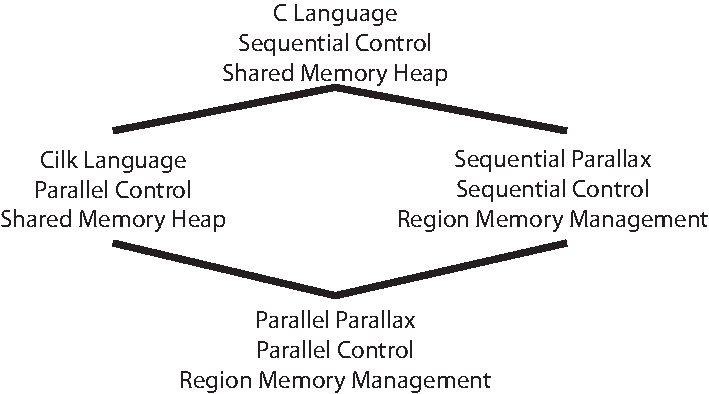
\includegraphics[width=3.5in]{figs/Taxonomy.pdf}
\caption{Relationship between tradition C, Cilk, and the sequential and
parallel versions of the Parallax language \label{fig:taxonomy}}.
\end{figure}

\subsection{Coherence Capabilities \label{Coherence}}
% Describe need for different ways of accessing regions
% Enables additional parallelism
% Tensor of coherence interactions
\noindent
In section \ref{Parallelism} we introduced mechanisms to create parallel computation
in Parallax.  We now need to present a memory model for understanding how
parallel operations can reason about memory accesses.  In this section we present
a memory coherency model for reasoning about the order of accesses to a single location
in memory.  In section \ref{Consistency} we describe a memory consistency model for
reasoning about the ordering of accesses to different locations. \\

\noindent
In most shared memory models coherence is maintained at the granularity of an address 
by hardware mechanisms.  This coherence model is not scalable and often times is 
overly restrictive.  In our approach coherence is maintained at the granularity of a 
region and can be controlled by the software.  Our approach to coherence allows us to
specify both how a function is going to access a region as well as who else is allowed
to access a region at the same time.  This will enable the compiler and runtime schedulers
to better exploit parallel work and only perform data movement when it is required. \\

\noindent
Our approach to memory coherence is governed by the idea of capabilities \cite{Stork09,Bierhoff07}.
Capabilities provide a type system solution to controlling access to a shared resource.
In our case the shared resource is access to a region and we want to manage how
computations are permitted to access it.  We extend our type system from section \ref{TypeSystem}
to now require every function declaration to be explicit about the capabilities required
for each region that will be accessed by the function.  When we go to type check the program
we enforce the following invariant: every statement in a function must require a subset of the
capabilities declared in the function declaration to be correct. \\

\noindent
The set of capabilities that can be acquired by a function is represented in a two dimensional
space.  The first dimension deals with how the function will access the region, while the
second dimension determines what other access may be permitted to the region while the function
is being executed.  This two dimensional space and the set of symbols that we use to represent
each can be seen in table \ref{tab:capabilities}.

\begin{table}
\centering
\begin{tabular}{|c||c|c|c|c|}
\hline
 & Exclusive & Atomic & Simultaneous & Relaxed \\ \hline \hline
Read-Only & ROE & ROA & ROS & ROR \\ \hline
Read-Write & RWE & RWA & RWS & RWR \\ \hline
Reduction(Write-Only)$<$op$>$ & WOE & WOA & WOS & WOR \\ \hline
\end{tabular}
\caption{Two dimensional space of coherence capabilities for regions and their symbols. \label{tab:capabilities}}
\end{table}

\noindent
Each row in table \ref{tab:capabilities} represents a different way that a function
might access a region.  If a function is only going to be reading values from a
region then it needs read-only capabilities.  If a function is going to be mutating
a region then it must have the region with read-write capabilities.  Finally if a
region is only going to be performing a reduction into a region then it needs
reduction capabilities. \\

\noindent
Each column in table \ref{tab:capabilities} corresponds to a different way in which
other functions are permitted to be accessing the region at the same time. 
\begin{itemize}
\item Exclusive - mandates that no other transactions may be using
the region in any form while the functions is accessing the region.
\item Atomic - other functions may be accessing the region at the same
time, but this function must appear to execute atomically (serializably) with respect
to other functions accessing the region.  This is equivalent to transactional memory semantics.
\item Simultaneous - other functions may be accessing the region at the
same time and all updates made by other functions MUST be made visible to the 
function accessing the region.  This is equivalent to traditional hardware
single-writer/multiple-reader coherence.
\item Relaxed - other functions may be accessing the region at the same time
and updates made by other functions MAY be visible to this function.  To force updates to be
visible there will be a set of memory operations (i.e. invalidate/flush) that
will be used to update values just like in software coherence schemes.
\end{itemize}

\noindent
By providing each of these different coherence capabilities we allow the programmer
to say explicitly what the coherence properties are of the function that is
being executed.  Ultimately this will allow us to extract as much parallelism
as possible from programs and to minimize the amount of memory movement that
might ultimately need to occur in machines with distributed hierarchical memory. \\

\noindent
We now have twelve possible memory coherence capabilities that can be requested
over two dimensions.  We now want to examine the concurrency rules for which
capabilities are able to be held by two functions executing at the same time.  Rather
than enumerate all 144 entries in this fourth-order tensor, we instead give rules
for which capabilities can held by different functions and these functions performed in parallel. 

\begin{itemize}
\item exclusive capabilities guarantee that now other function is accessing the region
\item atomic capabilities can only be used in conjunction with other functions which permit
serializability with the statements in those functions (strong isolation in TM terminology)
\item reduction operations can only be performed in parallel with reduction functions of
the same operand, otherwise they must be serialized
\end{itemize}

\noindent
It is important to note that for a sequential stream of statements to a region, all
capabilities must be acquired and released in the sequence of statements in the
program.  This guarantees classic sequential code guarantees.  However, outside
of this restriction, the compiler is free to re-order statements as desired as long
as the expected memory coherence behavior is respected.  The details of re-orderings
that are permitted are discussed in more detail in section \ref{Consistency}. 

\subsection{Memory Consistency Model \label{Consistency}}
% Weak consistency model based on location consistency, but on regions
% Add fences for guarantees 
\noindent
In section \ref{Coherence} we defined how capabilities could be used to
control the ordering of accesses to a single region.  In this section we deal
with the memory consistency model that describes what reordering of operations
are permitted across multiple regions.  Our view on memory consistency is
that Parallax is a low-level programming model that requires explicit input
from the programmer about the desired program output.  In conjunction with 
this view, we propose to use a very relaxed memory consistency model
called location consistency\cite{Frigo98}.   We will then provide additional
memory fence operations to the programmer to prevent unwanted reorderings.\\

\noindent
Traditionally memory consistency models have been defined over the set of
all addresses in a memory.  In our approach however, memory consistency
is now defined over the set of regions in a program.  While the number of
regions in this set is unbounded, in practice it is many orders of magnitude
smaller than total number of addresses available in a program.  This justifies
our choice to use a more relaxed memory model such as location consistency 
since the programmer will have many fewer reorderings to consider due to 
the limited number of regions in scope at any point in the program. \\ 

\noindent
Location consistency proposes that the only reorderings that are not permitted
are ones that would break the serial semantics of a serial execution of stream
of instructions.  We therefore must obey the serial set of operations to a region,
but reordering statements to different regions is acceptable.  This will come
in especially helpful in our implementation when it may be beneficial to overlap
computation with communication. \\

\noindent
In some cases the reordering of statements that side-effect different
regions is undesirable.  To avoid such cases the programmer can insert memory
fences.  Memory fences take an argument of either a region identifier or a region
collection to prevent any reordering of statements that affect those regions.  If
this argument list is left empty then no statements are permitted to be reordered
across the memory fence.   

\pagebreak

%%%%%%%%%%%%%%%%%%%%%%%%%%%%%%%%%%%%%%%%%%%%%%%%%%%%%%%%%%%%%%%%%%%%%%%%%%%%%%%%
% Mapping

\section{Mapping Parallax to Hierarchical Memory Machines \label{Mapping}}
% Tunables
% Adding tags to source code, separate mapping file for each architecture
% Complements dynamic runtime decision making
% Place constraints on functions and region instances
\noindent
Much like the original Sequoia language, Parallax will also use a mapping
file to specify how to map a Parallax program onto a given architecture.  Unlike
Sequoia's mapping file, the Parallax mapping file will provide more flexible
ways of performing this mapping and a different execution model for the
Parallax program.

\subsection{Tunable Parameters and Tagged Statements \label{Tunables}}
\noindent
Similar to Sequoia, Parallax allows for type declarations to be declared as
tunable variables.  These tunable variables will have their value fixed at 
a later time as specified by the Parallax execution model\footnote{This is different from
Sequoia where they had to be fixed at compile-time.}.  The tunable qualifier
can be applied to any plain-old-data (POD) type or to any function pointer.
The need for tunable function pointers is useful in the case where the algorithm
may either opt to recursively decompose a data structure, or perform the base computation.
In these scenarios a tunable function pointer can be used to represent both options. \\

\noindent
Unlike Sequoia tunable parameters can either be assigned explicit values or they
can be assigned a finite subset of values from which the compiler/runtime system
may choose.  These sets can either be specified in the original source code if they
are machine agnostic (i.e. some function pointers) or they can be specified in the
mapping file.  A mapping file must specify either a value or a set of values for every
tunable parameter in a source code or there will be a compile-time error.  This
ensures that the compiler/runtime will at least have a set of valid ranges over which
to perform a search if only a set is specified.\\

\noindent
In addition to specifying tunable variables, we also permit the programmer to tag
statements with labels as ways of providing a naming mechanism for use in the mapping
file.  By being able to tag statements, the programmer can add additional constraints
to the program that machine specific.  For example, a programmer can tag a {\tt spawn}
statement and in the mapping file indicate that for a specific machine the statement
must be executed in a {\tt must} context.  This would force the system to create
parallelism even if it potentially degraded performance.  The opposite would be to
tag a {\tt spawn} statement as a {\tt not} context in which case the compiler and 
runtime cannot create parallelism at this function call. \\

\noindent 
Tagged statements can also be used for specifying compiler and runtime plugins for
use with a specific statement as discussed in section \ref{Plugins}.

\subsection{Exact and Relative Mappings \label{ConstraintMap}}

\subsection{Compiler/Runtime Plugins \label{Plugins}}

\subsection{Constraint-Based Execution Model \label{Execution}}

\pagebreak

%%%%%%%%%%%%%%%%%%%%%%%%%%%%%%%%%%%%%%%%%%%%%%%%%%%%%%%%%%%%%%%%%%%%%%%%%%%%%%%%
% Outstanding Questions

\section{Outstanding Issues \label{OutstandingQs}} 
\noindent
Below are some issues that we have yet to resolve.
\begin{itemize}
\item Region Slicing: How do we describe region slicing for regions whose 
types are complex data types?  Are the regions created by region slicing 
still sub-regions?  How does this relate to the sub-region relationship?
\item What operations are supported on region collections?  Can region collections
be passed everywhere that a region identifier is passed?
\item How do we differentiate arrays form base region types?  Are there special
operations for arrays that we want to support that cannot be supported on
general regions?  Are these built-in operations?
\end{itemize}

\pagebreak

\bibliographystyle{IEEEtran}
\bibliography{parallax_model}

\end{document}
